% !TeX encoding = UTF-8
% !TeX spellcheck = en_US
% !TeX root = main_file.tex
\section{Tracking of UAV}
\subsection{Introduction}
There are several ways to track something using cameras and computer vision. One way is to look for the shape of the object of interest. Another way is to equip the object with a well known marker. 

A sufficiently advanced marker and program makes it possible for a single camera setup to deduce the orientation of the object (see \url{http://github.com/henrikmidtiby/markerlocator}), whereas a simple marker might only convey position ($x$, $y$). Knowing the marker size and the focal length allows for calculating the distance ($z$) to the object as well.

Identifying the object based on the profile of the object allows for deducing orientation ($\theta$) if the object is asymmetrical, position ($x$, $y$) and, using the focal length again, the distance ($z$). 

It was early on decided to use ROS as a framework for the vision program. This was done for a few reasons:
\begin{itemize}
	\item Previous experience with ROS
	\item Easy to add new functionality through ROS nodes
	\item Broad support for third party libraries
\end{itemize}

It was also decided to use OpenCV for the vision part, mainly because of previous experience. 

For the marker tracker, Henrik Midtiby’s MarkerLocator was investigated. While the system is quite clever, it proved too difficult to make it work as needed and to interface it with ROS, so a simplified marker tracker, which only tracks a circle, was implemented. In order to be able to deduce the orientation of the UAV, object tracking was implemented as well. Besides orientation, this solution was expected to give redundancy in position and distance estimation.
\subsection{ROS as a framework}
Using ROS as a framework can create confusion, when lots of nodes has been implemented. Therefore a overview of the desired nodes was drawn, with short descriptions of their functionality.
\begin{center}
	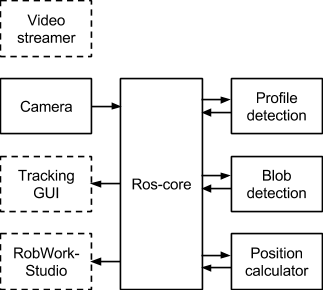
\includegraphics{imgs/ros_setup}
\end{center} 

\begin{center}
	\begin{minipage}[t]{0.20\textwidth}
		\textbf{Video streamer node}\\Publishes video from a video file. Designed for testing with video instead of video camera\\\\
		\textbf{Camera node}\\Publishes video from the camera
	\end{minipage}
	\hfill
	\begin{minipage}[t]{0.31\textwidth}
		\textbf{Tracking GUI node}\\Subscribes to video stream, profile- and blob-detection nodes. Shows the video stream with tracking information from the blob detection and profile detection nodes. \\\\
		\textbf{RobWorkStudio node}\\Subscribes to the position calculator node. Displays the the UAV position and landing pad in a 3D.
	\end{minipage}
	\hfill
	\begin{minipage}[t]{0.45\textwidth}
		\textbf{Profile detection node}\\Subscribes to the camera or video node. Tracks the position, size and orientation of the UAV and publishes the results.\\\\
		\textbf{Blob detection node}\\Subscribes to the camera or video node. Tracks the position and size of the marker and publishes the results.\\\\
		\textbf{Position calculator node}\\Subscribes to the profile- and blob-detection nodes. Calculates and publishes the UAVs 3D position in meters.
	\end{minipage}
\end{center}
\subsection{Tracking method}
\subsubsection{Blob detection}As mentioned a marker can be used or location the UAV. This marker were mounted at the bottom of the UAV as show in in the image below. 

\begin{center}
	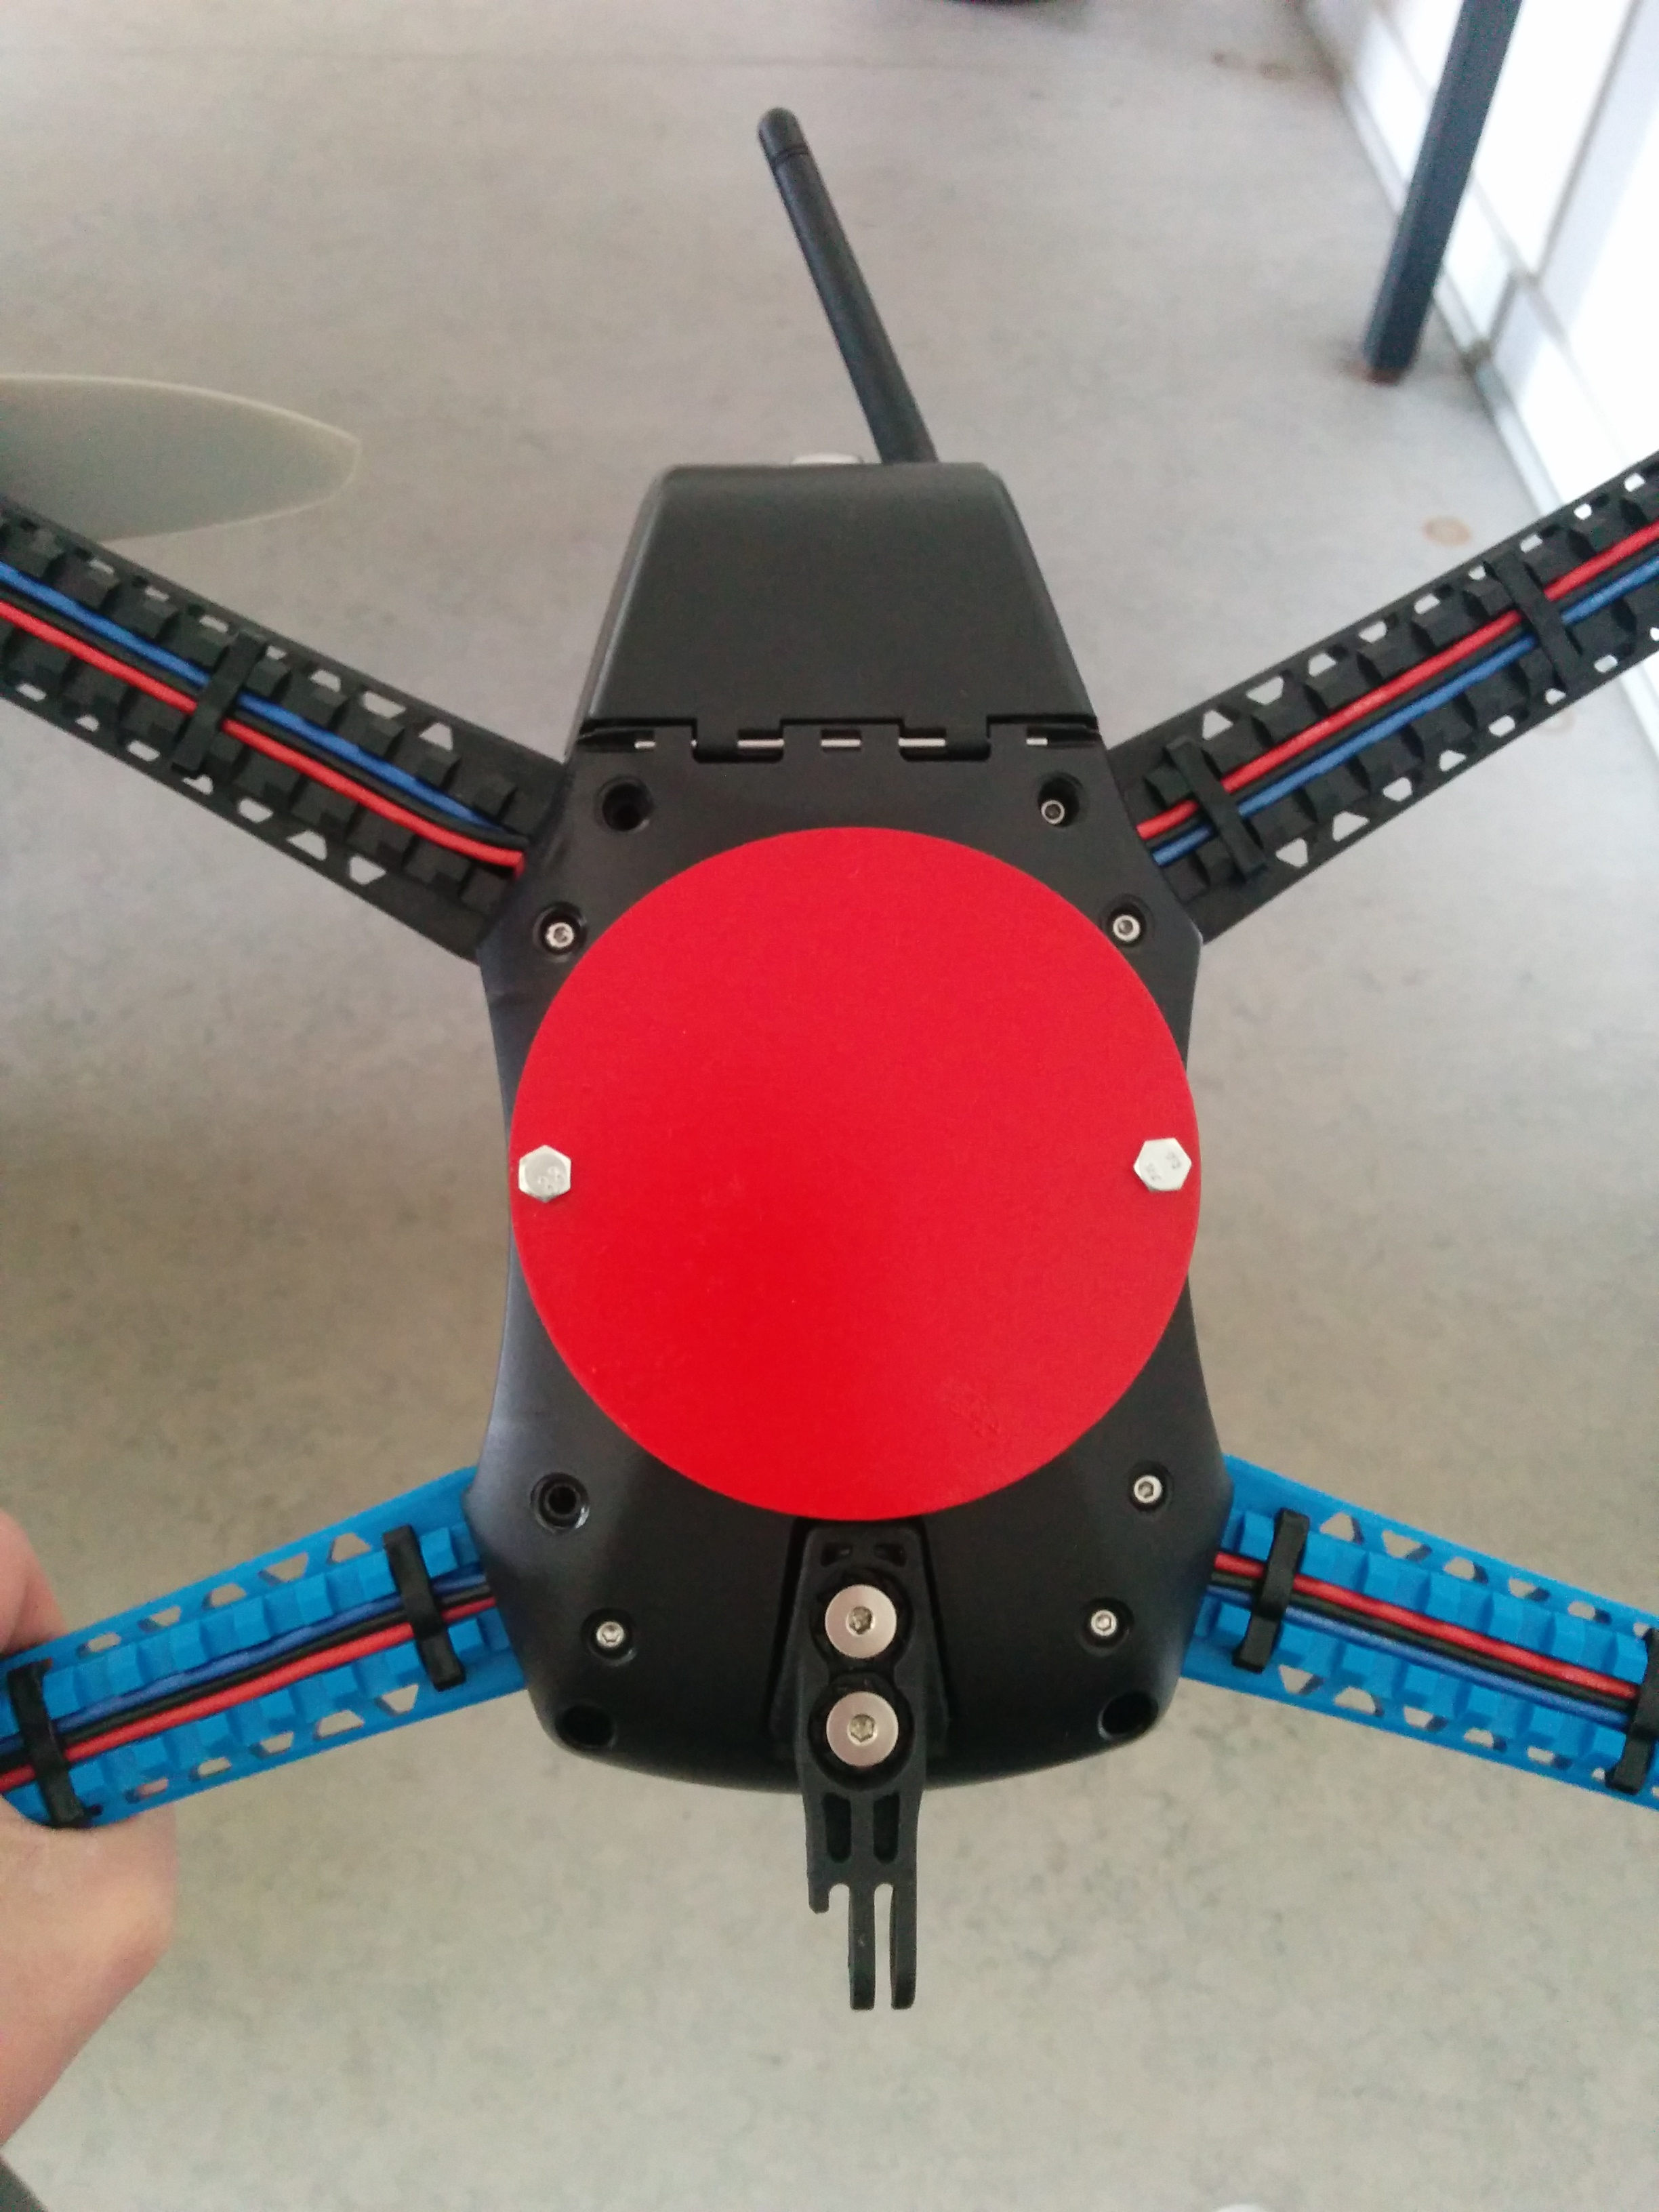
\includegraphics[width=0.4\textwidth, trim=15cm 15cm 12cm 23cm, clip=true]{imgs/blob_example}
\end{center}
The bright red color of the marker were chosen because it is easy to isolate in the image. 

it is possible to do so because a typical camera has three color channels. Red, green and blue. This means that we can remove pixels that doesn't have a clear red color by subtracting the blue and green color channels form the red. 
The result can be seen below.

\Huge
\textbf{Indsæt billede}
\normalsize\\
Only the marker and maybe a bit of noise is now left in the image, even though it is quite dark.
The last step is to locate the position and radius of the marker in the image. This was done by using OpenCV’s SimpleBlobDetector. It is a class containing function for extracting blobs radius and position from an image. It can even be configured only to locate round blobs, so noise and unexpected red object in the image won't give a false position.

\subsubsection{Profile (shape) detection}
Deducing the orientation of the UAV from detection of a circle would be, for a lack of better words, impossible. Postdoc at SDU-TEK Henrik Midtiby had developed a marker locator program (\url{https://github.com/henrikmidtiby/markerlocator}), but it didn’t work as expected. Specifically, with the tested implementation the marker identifiers in the image would find a random edge and stay there; if the marker was moved to the edge, the identifier would assume the edge of the paper, on which the marker was, to be the edge to follow. Only by forcing the identifiers to touch the marker did they find the marker; but once the marker was identified, the identifiers worked flawlessly. 

Starting the marker locator with the marker in the image gave a completely different result, where the marker was located immediately. However, having to force the marker locator like that to get the orientation of the UAV would be cumbersome; having to shut down the program until the marker was correctly identified was equally cumbersome (mostly because there was no way to be sure that the found edge belonged to the marker). Henrik Midtiby, while trying to help out with usage of his marker locator, mentioned that using the UAV in itself rather than a marker could prove beneficial.

Since the UAV has a dark profile on the background of the bright sky, isolating the UAV through ordinary computer vision is done in simple steps. Below is pseudo code showing the process of finding the UAV; it is assumed that the shape of the UAV is already identified and loaded into the program.

\begin{center}
	\begin{minipage}[t]{0.1\textwidth}
		\begin{flushright}
			Lineno.\\1\\2\\3\\4\\5\\6\\7\\8\\9\\10\\11\\12\\13\\14
		\end{flushright}
	\end{minipage}
	\begin{minipage}[t]{0.8\textwidth}
		~\\input-image \textbf{Img}\\
		original-shape \textbf{OrgShape}\\
		blur(\textbf{Img})\\
		erode(\textbf{Img})\\
		binary\_threshold(\textbf{Img})\\
		erode(\textbf{Img})\\
		dilate(\textbf{Img})\\
		findContours(\textbf{Img}) => \textbf{NewShapes}\\
		matchShapes(\textbf{NewShapes}, \textbf{OrgShapes}) => \textbf{Matches}\\
		min(\textbf{Matches}) => \textbf{BestMatch}\\
		center(\textbf{BestMatch}) => \textbf{X}, \textbf{Y}\\
		orientation(\textbf{BestMatch}) => \textbf{Orientation}\\
		distance(\textbf{BestMatch}) => \textbf{Distance}\\
		return(\textbf{X}, \textbf{Y}, \textbf{Orientation}, \textbf{Distance})
	\end{minipage}
\end{center}
Lines 1--2 declares the two objects to compare. Lines 3--4 prepares the image for thresholding. Line 5 performs binary threshold to ease the object recognition. Lines 6--7 removes left over noise, such as birds, by first shrinking objects and then enlarging them. Then, in line 8, the built in OpenCV function findContours is applied to the image which results in a list of objects in the image. This list is compared to the known shape in line 9, resulting in a list of numbers; the lower the number the better the match. Line 10 shows how the best match is found. Lines 11--13 shows how the center, orientation and distance, all in pixels, are found. Line 14 returns the found values.

The program was developed using a video shot indoors. The image which is used as the original shape (line 2) is extracted from that video. Since the lighting is different indoors and outdoors, the program relies on a slower shutter speed than what was the case once the camera was moved outdoors. The camera is a standard web camera with a rolling shutter; this means that the propellers has strange contorted shapes outdoors rather than moving so fast compared to the indoors shutter speed that they are blurred away. 

This means that the program can have some problems identifying the correct shape. An experiment showed that while the UAV is located very often, the propellers and occasional bird can prove problematic when the UAV is close to the camera. Worst case observed behavior is 6 out of 55 frames being wrong, or 11 \% error rate, with the calculated distance to camera being 116 to \SI{138}{\centi\meter}. Out of the wrong frames, 3 was with no shape detected and 3 was the wrong shape. Best case observed behavior is 1 out of 130 frames being wrong, or 0.7 \% error rate, with calculated distance being 289 to \SI{415}{\centi\meter}. The single wrong frame was due to no shape detected.
\subsection{Position calculator}
When the UAV position in the image is known, it is possible to calculate its x, y, z position in the real world. This can be done because the radius of the UAV/marker in the real world and in the image is known. 

First the direct distance from camera to the UAV/marker can be calculated. This is done by using the camera model as shown below.
\begin{figure}[h!]
	\centering
	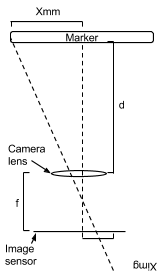
\includegraphics{imgs/focal_length}\\
	d = distance to UAV (\si{\milli\meter})\\
	Ximg = radius of the UAV/marker on the image (pix)\\
	Xmm = real world radius of UAV/marker\\
	f = focal length of the camera
\end{figure}

There are two unknowns in the model above, the focal length and the distance to the UAV. The focal length is a constant that is dependent on the camera, so it can be measured, and used to calculate the distance in the future. 
It is found by placing the marker in a known distance from the camera, and then simply calculating it using the camera model.

\begin{figure}[h!]
	\centering
	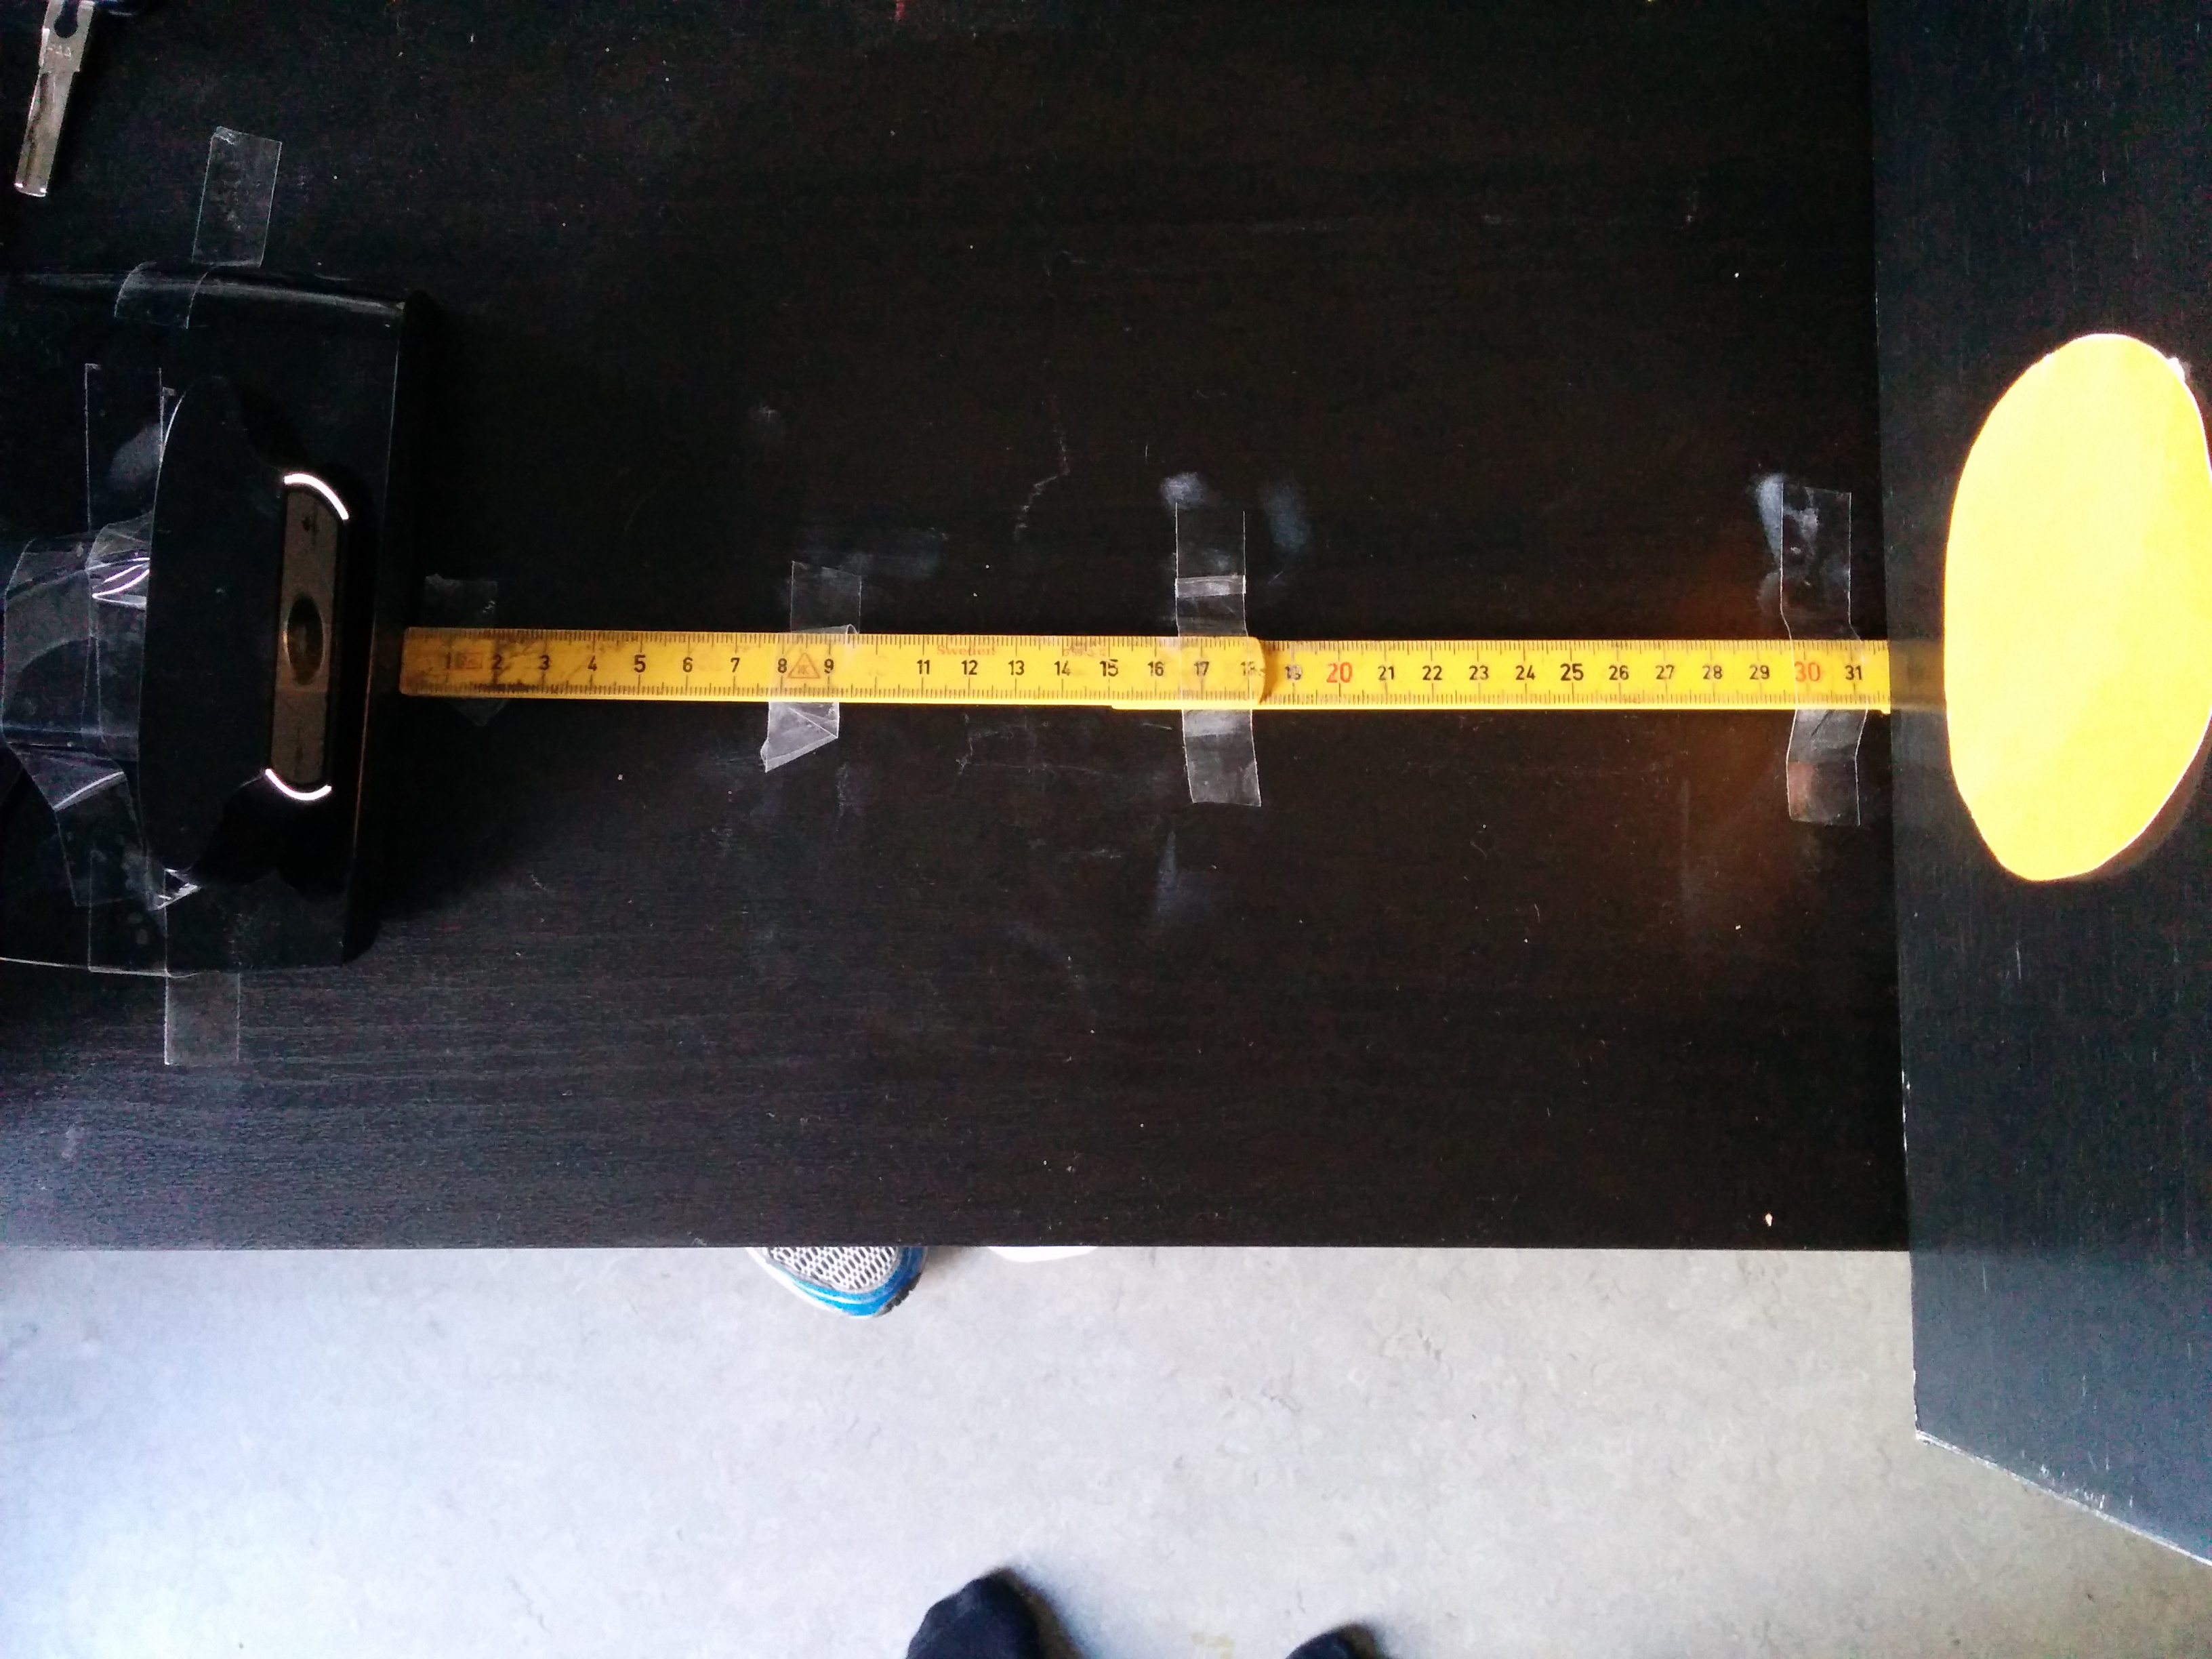
\includegraphics[width=0.8\textwidth]{imgs/focal_length_test}
	\caption{Test setup for measuring the focal length}
\end{figure}

Now that the distance to the UAV is known, it's possible to find the distance on the z-axis. The z axis is pointing directly out of the camera, and is equivalent the altitude of the UAV, when the camera is looking directly upwards. 

\begin{figure}[h!]
	\centering
	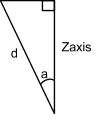
\includegraphics{imgs/focal_length_z_length}\\
	a = pixelsformcenter\! $ \times \frac{1}{14.2}$(pix/deg)\\
	Zaxis = $\frac{\mathrm{d}}{\cos{(a)}}$
\end{figure}

The $\frac{1}{14.2}$ actor above is the width of the image divided by the camera's view angle, giving the unit pixels/degree.

When angle $a$ is known, the cosine-relationships can be used to calculate the distance in the z-axis.

This leads us to the final step. Calculating the distance in the x- and y-plane.
 
Since the distance in the z-plane is known, it's possible to rewrite and use the formulas for calculating the distance to the UAV. 

Replacing the distance to the UAV with the distance on the z-axis, and using the pixel distance from the center (in the x, y axis) instead of the marker/UAV radius gives the equations below.

\begin{align}
X\mathit{pix}&= \frac{f}{Z\mathit{mm}}\times X\mathit{mm} &\Rightarrow X\mathit{mm}=\frac{X\mathit{pix}\times Z\mathit{mm}}{f}\nonumber\\
Y\mathit{pix}&= \frac{f}{Z\mathit{mm}}\times Y\mathit{mm} &\Rightarrow Ymm=\frac{Ypix\times Zmm}{f}\nonumber
\end{align}
\begin{center}
	Xmm/Ymm = distance on the x or y axis\\
	Xpix/Ypix = pixel distance on the x or y axis in the image\\
	Zmm = distance on the z axis (altitude)
\end{center}
\subsection{Test}
All Ros tracking components were tested separately by use of the video streamer node, making unit testing easy.

At last the system where test together. A video demo of the full tracking system can be seen at \url{https://youtu.be/I4g7Ij-pmPY}.
\begin{figure}
	\centering
	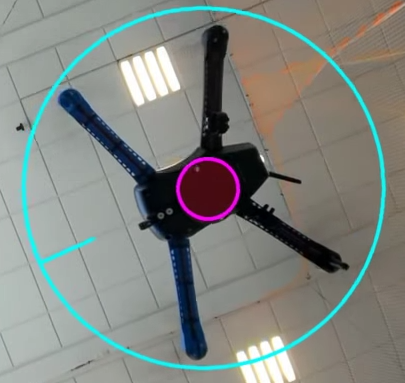
\includegraphics[width=0.8\textwidth]{imgs/tracking-test-indoors}\\
	Image from test\\Pink circle: Marker detection\\
	Blue circle: Profile detection\\Blue line: Orientation from profile detection
\end{figure}
\subsection{Part conclusion}
Due to the brightness of the sky, the blob detection does not work well outdoors at the tested distances. As a matter of fact, it does not work at all at the tested distances. Indoors detection works much better, as exemplified in the picture above. 

The shape detector works considerably better, and possibly good enough for actual implementation in a finished product. A better camera might be able to see the blob, allowing for all parts of the visual tracking system to work.